
\documentclass[a4paper,11pt]{article}
\usepackage{graphicx}
\usepackage{wrapfig}
\newcommand{\gtrsim}{\lower.5ex\hbox{$\; \buildrel > \over \sim \;$}}
\newcommand{\lesssim}{\lower.5ex\hbox{$\; \buildrel < \over \sim \;$}}
\newcommand\farcs{\mbox{$.\!\!^{\prime\prime}$}}% 
\pagestyle{empty}
\setlength{\topmargin}{-25mm}
\setlength{\textheight}{270mm}
\setlength{\textwidth}{180mm}
\setlength{\oddsidemargin}{-10mm}
\setlength{\evensidemargin}{-10mm}
\begin{document}

\begin {centering}
{\bf The Substructure Mass Function From an Unusually Magnified Quasar Host} {\bf (PI: Rusu C.E.)}\\
 \end{centering}
 
\medskip

\noindent {\bf Abstract.} The recently discovered quadruply lensed quasar SDSS~J1640+1932 ($z_\mathrm{lens}=0.20, z_\mathrm{QSO}=0.78$; Wang et al. 2017, MNRAS 468, 3757; fig. 1, left) has a spectacularly magnified host galaxy stretched into a $5''$-diameter Einstein ring. This is only the second system where dark matter substructure around a single massive elliptical galaxy can be searched for in high detail (low masses $\sim10^8$ $M_\odot$) based on conjoined constraints from perturbations to the Einstein ring as well as flux ratio anomalies. Adaptive optics imaging is key to using the information contained in the extended Einstein ring to detect low-mass substructure in this system, and to ultimately set constraints on the substructure fraction and mass function of dark matter.

$\Lambda$CDM has been remarkably successful in the large-scale linear regime, where density fluctuations are small. However, in the non-linear, high-density regime, observations and theory appear to diverge. Simulations predict a large amount of substructure, with $f_\mathrm{sub}$=5-10\% of the total halo mass within the virial radius being in substructures of $4\times10^{6-9} M\odot$, and with a substructure mass function of $dN/dm\propto m^{-\alpha}$, where $\alpha=1.9\pm0.1$ (e.g., Diemand et al. 2007, ApJ, 667, 859). However, for the luminous satellites in the Milky Way, $\alpha\sim1$ even after recent discoveries of low-luminosity satellites (e.g., Zucker et al. 2006, ApJL, 650, L41). To build up meaningful statistics requires that we more precisely quantify sub-galactic substructure distributions in other galaxies, not only in the Local Group, which may be a special case. 

Gravitational lensing provides a uniquely powerful approach to this problem, because it does not require the substructures to be luminous, and gives a direct measurement of the masses of detected substructure. Traditionally, flux ratio anomalies in lensed quasars have been used to statistically measure the level of substructure in distant galaxies (e.g., Metcalf et al. 2002, ApJ, 567, L5 ), but Vegetti et al. 2012 (Nature, 481, 341) has generalized this to ``surface brightness anomalies'' in Einstein rings (fig. 1, center), managing to place meaningful, although still loose constraints, on both $f_\mathrm{sub}$ and $\alpha$ (fig. 1, right). Excluding RX~J1131-1231, SDSS~J1640+1932 is the only lensed quasar where the host galaxy is stretch over a large radial region around an elliptical galaxy, and is therefore ideal to improve the available constraints on $f_\mathrm{sub}$ and $\alpha$.

\begin{minipage}{\textwidth}
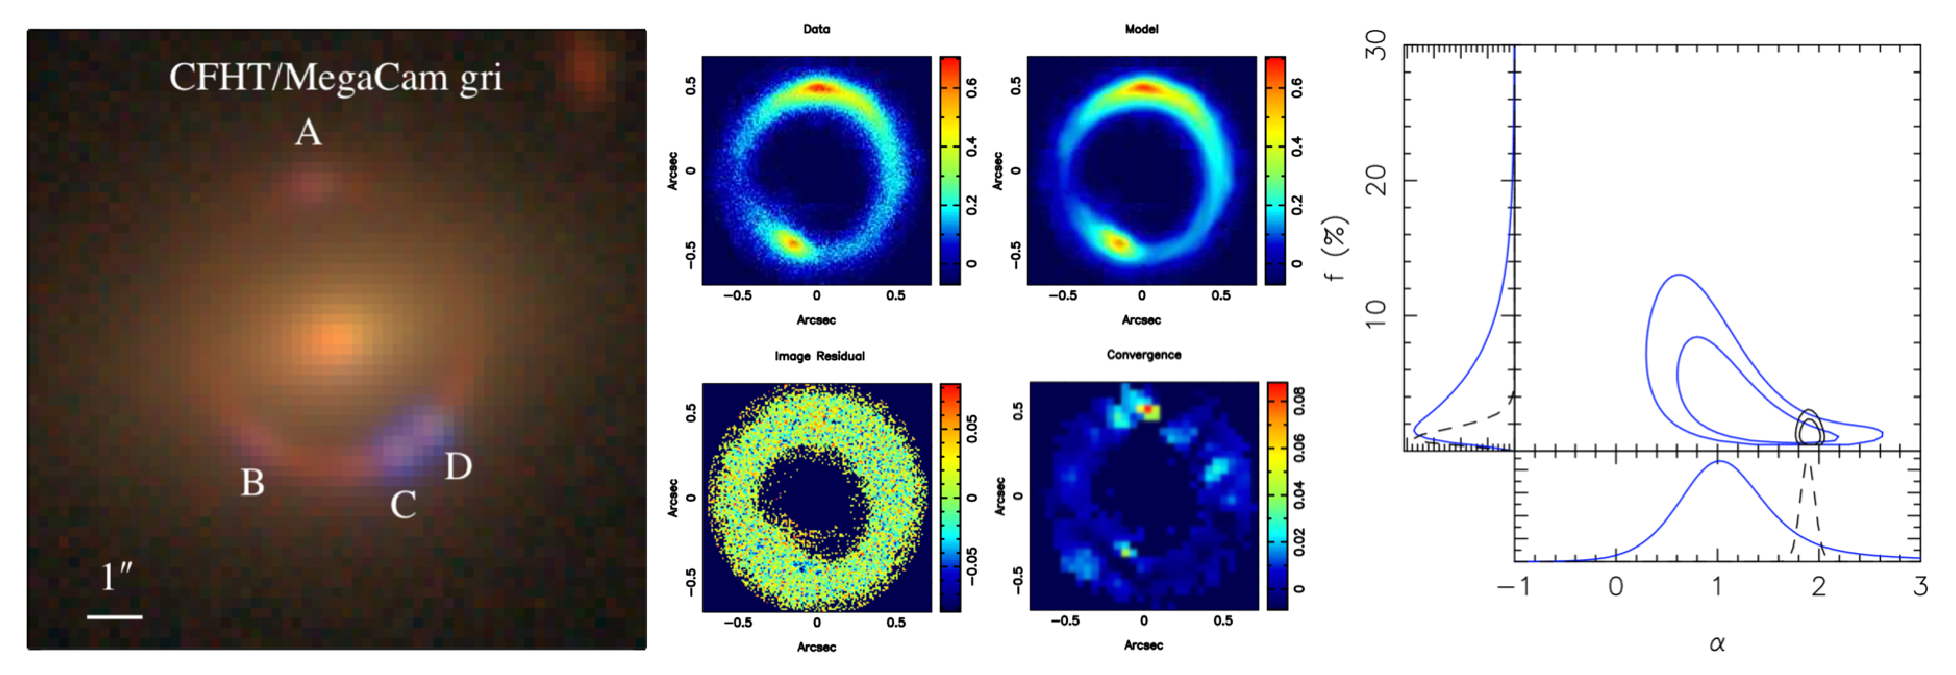
\includegraphics[width=0.95\hsize]{collage.eps}
\end{minipage}
Fig. 1: {\it Left:} CFHT image of SDSS~J1640+1932 (Wang et al. 2017). {\it Center:} Detection of a substructure based on Einstein ring modeling in the B1938+666 lens (Vegetti et al. 2012). The convergence map (lower right panel) is essentially a correction to the mass surface density map. The dark substructure shows up as the convergence peak at the top of the ring. {\it Right}. Conjoined constraints on $f_\mathrm{sub}$ and $\alpha$ from a single lens (Vegetti et al. 2012). The dashed contours are the results obtained when applying a Gaussian prior on $\alpha$ from a second lens system.

{\bf Ancillary Science.} I will use the highly detailed reconstruction of the quasar host galaxy, a byproduct of this work, to obtain a detailed lens galaxy mass model and use it to infer $H_0$ using the time-delay method (Bonvin et al. 2017, MNRAS, 465, 4914), pending low-resolution monitoring. I will also use the reconstructed host  to study the relation (if any) between the supermassive black hole and the stellar mass/luminosity of its late-type host galaxy at intermediate redshift (e.g., Ding et al. 2017, MNRAS, 472, 90). 

{\bf This Proposal.} I propose to obtain SDSS~J1640+1932 imaging with IRCS+AO188+LGS, in order to model in high detail the extended Einstein ring and look for low mass substructure. I will perform the analysis using the recently released code \texttt{lenstronomy} (Birrer et al. 2018, arXiv:1803.09746). Observations in both $H$ and $Ks$ filters will allow to cross-check any potential substructure detections, and to rule out false positives caused by extinction in the host. I will also measure for the first time in this system quasar image flux ratios unaffected by optical microlensing, and use the potential flux anomalies as a second probe of substructure. Finally, I will combine the results (including non-detections) with those from the previously analyzed handful of systems such as B1938+666 and RX~J1131-1231, in order to improve the existing constraints on $f_\mathrm{sub}$ and $\alpha$.

\end{document}
